\documentclass[12pt,a4paper]{article}
\usepackage[utf8]{inputenc}
\usepackage[spanish]{babel}
\usepackage{amsmath,amssymb}
\usepackage{graphicx}
\usepackage{geometry}
\usepackage{hyperref}
\usepackage{xcolor}
\usepackage{fancyhdr}

\geometry{top=2.5cm,bottom=2.5cm,left=2.5cm,right=2.5cm}

% Configuración de encabezados y pies de página
\setlength{\headheight}{14.5pt}
\addtolength{\topmargin}{-2.5pt}
\pagestyle{fancy}
\fancyhf{}
\rhead{Fundamentos de Inteligencia Artificial}
\lhead{Reporte Técnico}
\cfoot{\thepage}
\renewcommand{\headrulewidth}{0.4pt}
\renewcommand{\footrulewidth}{0.4pt}

\begin{document}

% --- INICIO DE LA PORTADA ---
\begin{titlepage}
    \begin{figure}[ht]
       \begin{minipage}{0.65\textwidth}
            
\includegraphics[width=4cm]{figs/LogoUPV.jpeg}
       \end{minipage}
       \begin{minipage}{0.3\textwidth}
            
\includegraphics[width=4cm]{figs/UTYP.jpeg}
       \end{minipage}
    \end{figure}
    
    \vspace{0.5cm}
    
    \begin{center}
        {\Huge \textbf{Universidad Politécnica de Victoria}}\\[1cm]
        
        {\LARGE \textbf{Asignatura:} Fundamentos de Inteligencia Artificial}\\[1.5cm]
        
        {\Large \textbf{Actividad 1:}}\\[0.5cm]
        {\huge \textbf{Configuración de entorno de desarrollo}}\\[2cm]
        
        {\Large \textbf{Elaborado por:}}\\[0.5cm]
        {\Large Junior Arturo Vázquez Leonel - 2430319}\\[1.5cm] % Cambiar por los datos reales
        
        {\Large \textbf{Docente:}}\\[0.5cm]
        {\Large Dr. Said Polanco Martagón}\\[2cm] % Cambiar por los datos reales
        
        \vfill
        
        {\large \today}\\[1cm]
    \end{center}
\end{titlepage}
% --- FIN DE LA PORTADA ---

\section{Configuración del Entorno de Desarrollo}
A continuación se presenta la evidencia de la instalación del entorno virtual y los paquetes necesarios.

\begin{figure}[htbp]
    \centering
    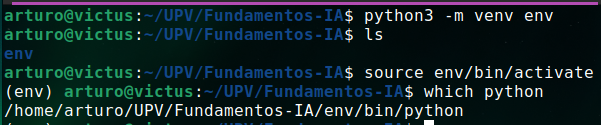
\includegraphics[width=0.9\textwidth]{figs/Intalacion Entorno.png}
    \caption{Captura de pantalla de la instalación del entorno de desarrollo.}
\end{figure}

\section{Prueba de Importación de Librerías}
A continuación se muestra la captura de pantalla de la consola/notebook ejecutando la prueba de importación de las librerías solicitadas.

\begin{figure}[htbp]
    \centering
    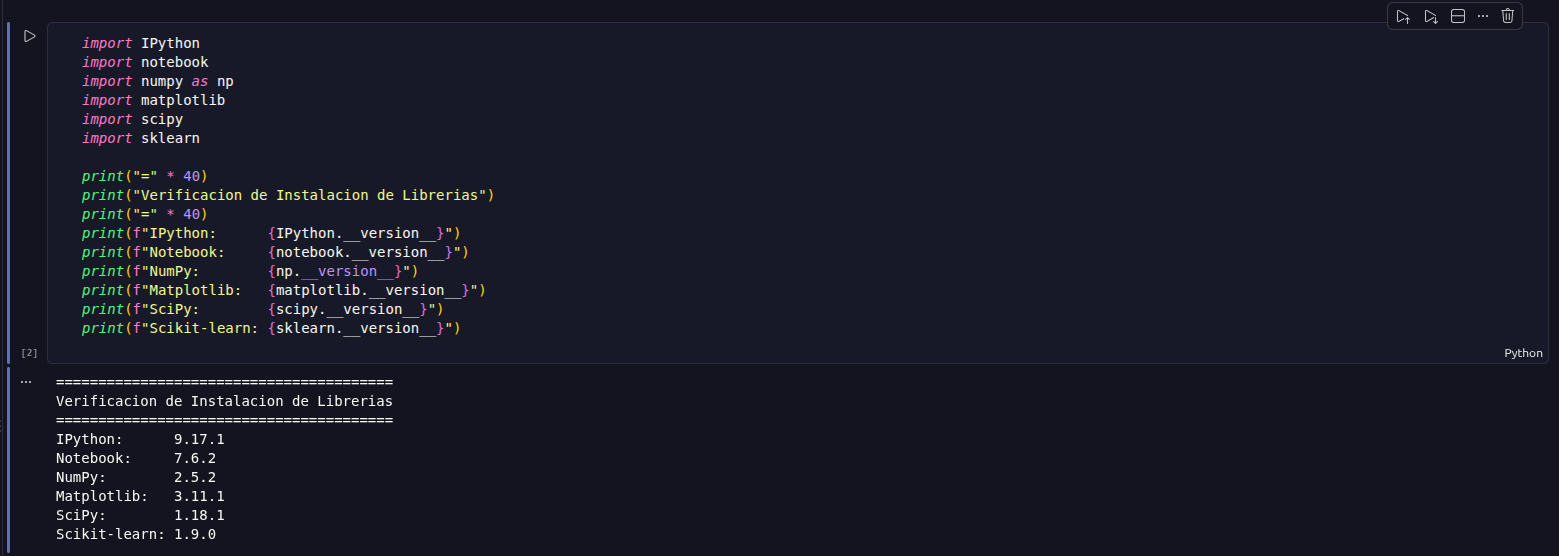
\includegraphics[width=0.9\textwidth]{figs/Instalacion Librerias (Visual Studio View).png}
    \caption{Captura de pantalla de la ejecución y prueba de importación.}
\end{figure}

\section{Investigación Técnica: Python en la Ingeniería e Innovación Digital}

\begin{figure}[htbp]
    \centering
    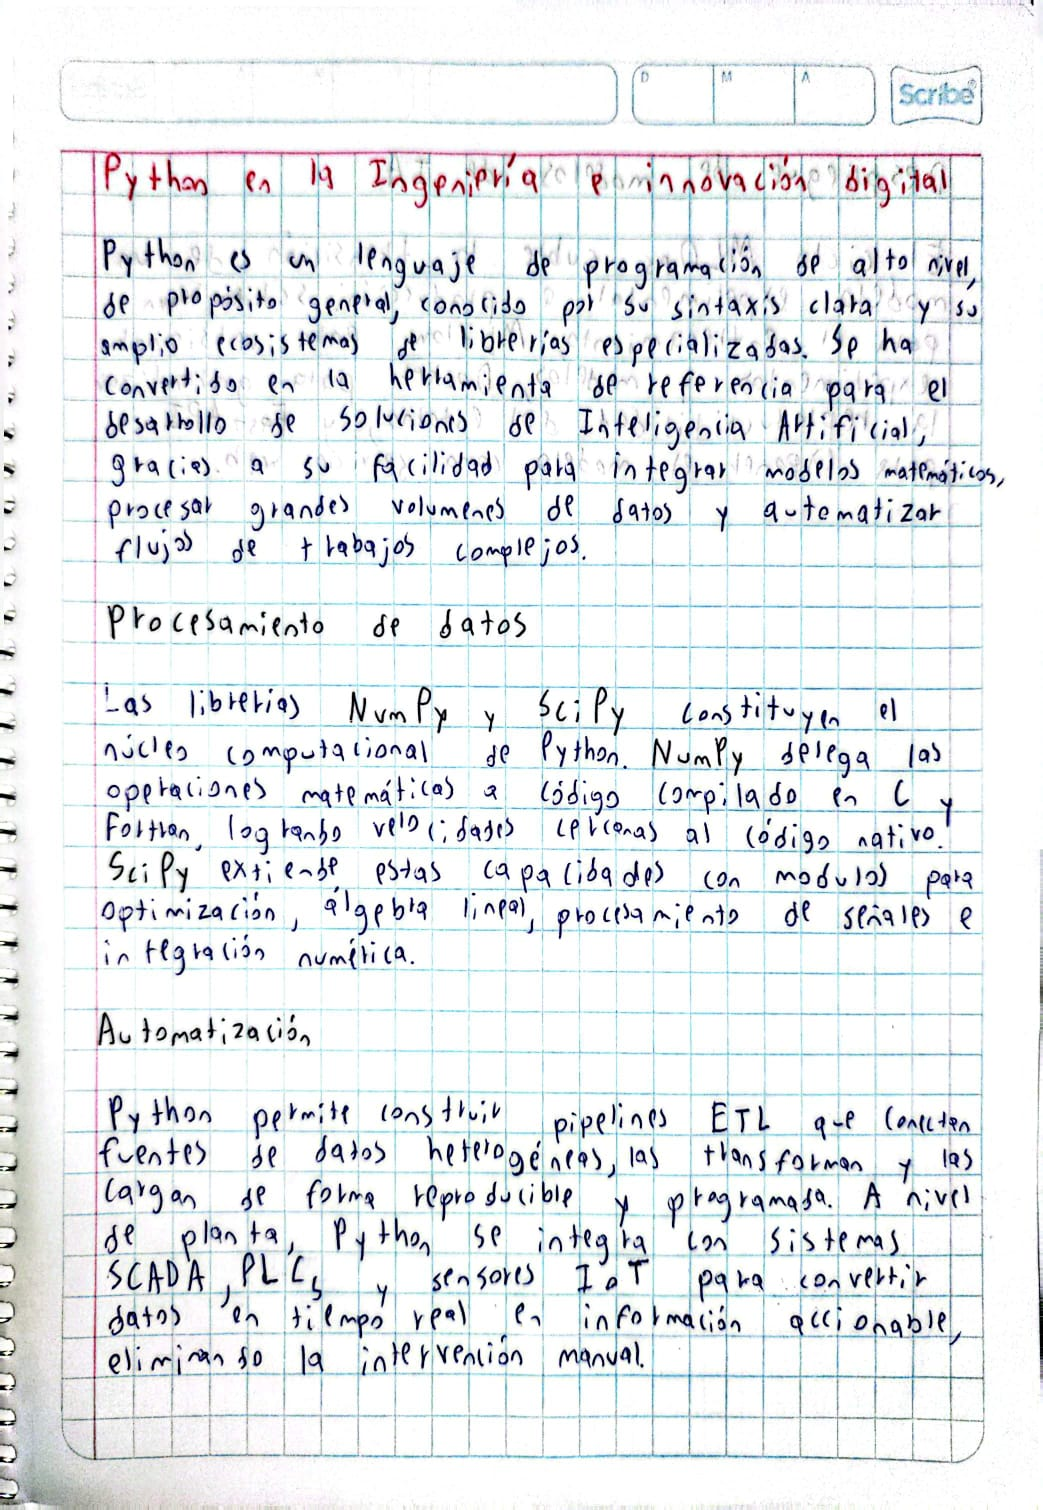
\includegraphics[width=0.75\textwidth]{figs/Investigacion_p1.jpeg}
    \caption{Investigación técnica manuscrita (Parte 1).}
\end{figure}

\begin{figure}[htbp]
    \centering
    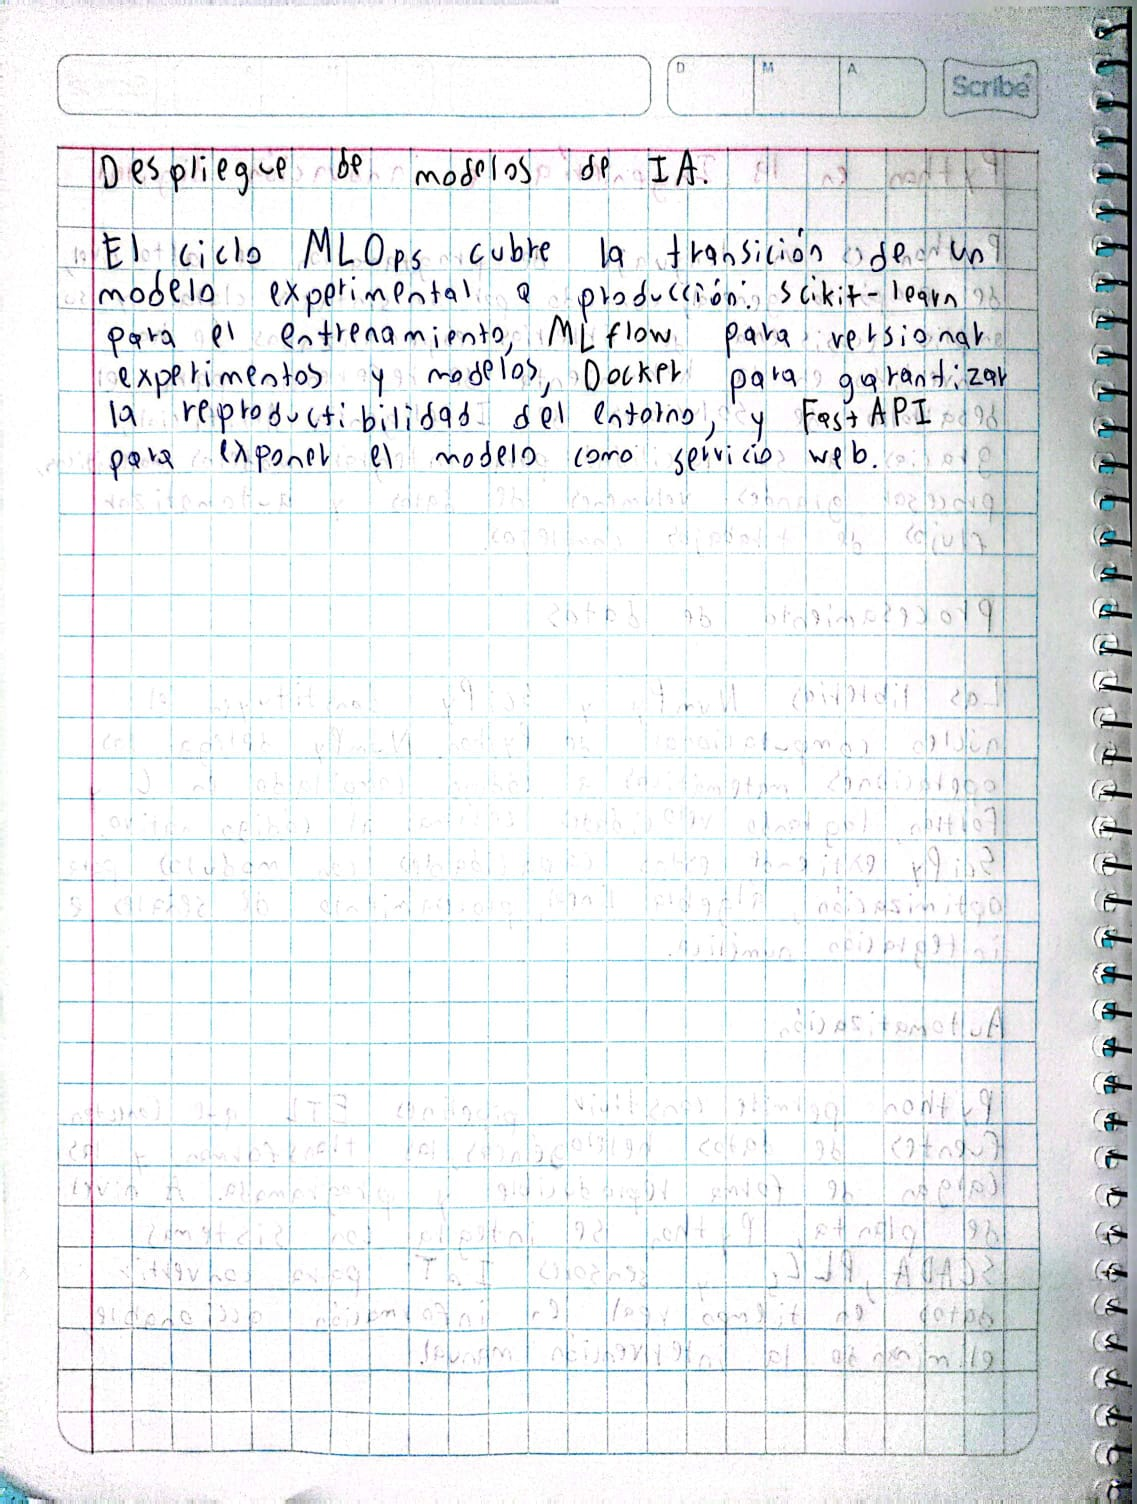
\includegraphics[width=0.75\textwidth]{figs/Investigacion_p2.jpeg}
    \caption{Investigación técnica manuscrita (Parte 2).}
\end{figure}

\end{document}
